\documentclass[aspectratio=169,12pt]{beamer}
\usepackage[T1]{fontenc}
\usepackage{lmodern,booktabs,tikz}
\definecolor{Ink}{HTML}{17324D}
\definecolor{Teal}{HTML}{007F7B}
\definecolor{Gray}{HTML}{697887}
\definecolor{Soft}{HTML}{EEF3F6}
\setbeamercolor{normal text}{fg=Ink,bg=white}
\setbeamercolor{frametitle}{fg=Ink}
\setbeamercolor{structure}{fg=Teal}
\setbeamercolor{block title}{fg=white,bg=Teal}
\setbeamercolor{block body}{fg=Ink,bg=Soft}
\setbeamertemplate{navigation symbols}{}
\setbeamersize{text margin left=9mm,text margin right=9mm}
\setbeamerfont{frametitle}{size=\Large,series=\bfseries}
\newcommand{\evidencecutoff}{\ifnum\insertframenumber=4 05:30\else 01:14\fi}
\setbeamertemplate{footline}{\hspace{9mm}\scriptsize Exploratory update | 29 September 2026 | Cutoff \evidencecutoff\ UTC\hfill\insertframenumber/5\hspace{9mm}\vspace{3mm}}
\newcommand{\aside}[1]{\vfill{\footnotesize\color{Gray}#1\par}}
\hypersetup{pdftitle={Teaching usable next steps: research update, 29 September 2026},pdfauthor={Alex Towell}}
\begin{document}

\begin{frame}[t]
\frametitle{Good examples should teach usable next steps.}
To tackle an unfamiliar goal, a model must find missing information, choose smaller steps and use tools correctly.
\begin{block}{Our test is TextCraft, a crafting game.}
The model looks up recipes, makes parts and assembles the requested items. The game checks whether it made the right quantities, not whether its answer sounds convincing.
\end{block}
Our longer-term aim is a recursive language model: it can ask another model to solve a useful part of the task.
\medskip

First, can better worked examples teach decisions that make sense from what the model has seen?
\aside{The teaching and reward-training results here use one small model family, Qwen3-4B. They do not establish that recursion helps.}
\end{frame}

\begin{frame}[t]
\frametitle{Introduce a part before asking about it.}
Supervised fine-tuning (SFT) teaches the model to copy the next action.
\vspace{2mm}
\begin{center}
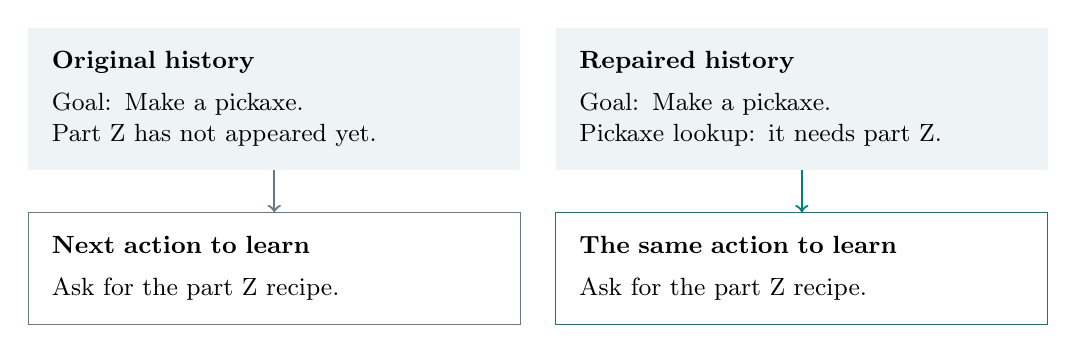
\begin{tikzpicture}[font=\small]
\node[anchor=north west,align=left,text width=5.65cm,fill=Soft,inner sep=3mm] (before) at (0,0) {\textbf{Original history}\\[1.5mm]Goal: Make a pickaxe.\\Part Z has not appeared yet.};
\node[anchor=north west,align=left,text width=5.65cm,fill=Soft,inner sep=3mm] (after) at (6.7,0) {\textbf{Repaired history}\\[1.5mm]Goal: Make a pickaxe.\\Pickaxe lookup: it needs part Z.};
\node[anchor=north west,align=left,text width=5.65cm,draw=Gray,inner sep=3mm] (beforeanswer) at (0,-2.35) {\textbf{Next action to learn}\\[1.5mm]Ask for the part Z recipe.};
\node[anchor=north west,align=left,text width=5.65cm,draw=Teal,inner sep=3mm] (afteranswer) at (6.7,-2.35) {\textbf{The same action to learn}\\[1.5mm]Ask for the part Z recipe.};
\draw[->,thick,Gray] (before.south)--(beforeanswer.north);
\draw[->,thick,Teal] (after.south)--(afteranswer.north);
\end{tikzpicture}
\end{center}
The repair changes lookup order and input histories, not the taught answers or number of training steps.
\aside{Illustration only. The repair uses a known correct action list; it is not a discovery planner.}
\end{frame}

\begin{frame}[t]
\frametitle{The repair helped in three small comparisons.}
Successes out of 32; the taught answers and number of training steps stay fixed.
\vspace{1mm}
\begin{center}
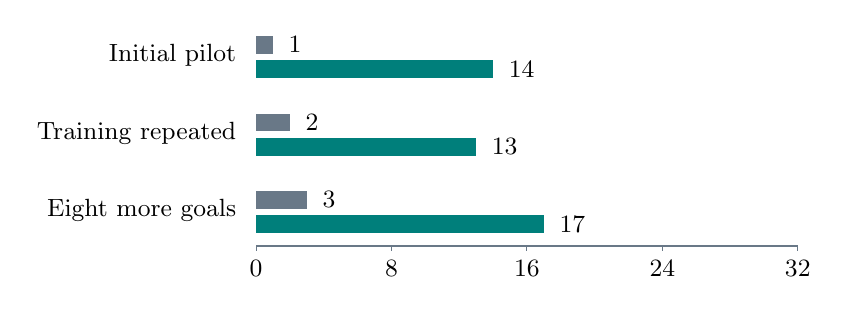
\begin{tikzpicture}[x=.215cm,y=.41cm,font=\small]
\node[anchor=east] at (-.6,5.35) {Initial pilot};
\node[anchor=east] at (-.6,2.95) {Training repeated};
\node[anchor=east] at (-.6,.55) {Eight more goals};
\fill[Gray] (0,5.4) rectangle (1,5.95);
\fill[Teal] (0,4.65) rectangle (14,5.2);
\fill[Gray] (0,3) rectangle (2,3.55);
\fill[Teal] (0,2.25) rectangle (13,2.8);
\fill[Gray] (0,.6) rectangle (3,1.15);
\fill[Teal] (0,-.15) rectangle (17,.4);
\node[anchor=west] at (1.35,5.68) {1};
\node[anchor=west] at (14.35,4.93) {14};
\node[anchor=west] at (2.35,3.28) {2};
\node[anchor=west] at (13.35,2.53) {13};
\node[anchor=west] at (3.35,.88) {3};
\node[anchor=west] at (17.35,.13) {17};
\draw[Gray] (0,-.55)--(32,-.55);
\foreach \n in {0,8,16,24,32} {\draw[Gray] (\n,-.55)--(\n,-.7);\node[below,font=\small] at (\n,-.7) {\n};}
\end{tikzpicture}
\end{center}
{\small\color{Gray}\rule{4mm}{2mm} Original examples\qquad\color{Teal}\rule{4mm}{2mm} Repaired examples}
\medskip

{\small Each row repeats eight goals in two recipe worlds, twice per world. The first two rows reuse the same goals. These are exploratory, previously examined panels.}
\aside{Input lengths differ; extra training partly rescues the original examples. This tests limited training budgets.}
\end{frame}

\begin{frame}[t]
\frametitle{Reward training showed little transfer.}
Reinforcement learning (RL) rewards task completion. We trained once for each tool setting. Successes before $\to$ after, out of 16:
\vspace{3mm}
\begin{center}
\renewcommand{\arraystretch}{1.25}
\begin{tabular}{lcc}
\toprule
Tool setting & Familiar goals & Different goals\\
\midrule
Model supplies ingredients & $9 \to 13$ & $4 \to 5$\\
Code fills known ingredients & $14 \to 16$ & $5 \to 5$\\
\bottomrule
\end{tabular}
\end{center}
\medskip

Each column: eight goals, two attempts each. The different target items were not used in training, but share the same recipe world.
\medskip

Different goals: one extra success without assistance, none with it.
\aside{Code uses only observed recipes. Learning on a new training-goal set and comparison with more example-based training are still pending.}
\end{frame}

\begin{frame}[t]
\frametitle{Next, test transfer and the value of one helper.}
\begin{block}{Does the teaching repair work in another model family?}
We will train a second kind of model, Phi-4-mini, on the repaired examples. That test is still pending.
\end{block}
\begin{block}{Does a helper improve the whole task?}
We will compare one helper with working alone, under the same total allowance for calls and generated text.
\end{block}
A helper completed a subtask, but the short test stopped before we could assess the whole task.
\medskip

\textbf{For discussion:} Which result would most change your confidence in this approach?
\aside{No whole-task helper benefit or general recursive reasoning has been demonstrated.}
\end{frame}
\end{document}
